\documentclass[a4paper,12pt,oneside]{book}
\usepackage{graphicx}
\usepackage{fancyhdr}
\usepackage[font = scriptsize, bf]{caption}
\usepackage[italian]{babel}
\usepackage[latin1]{inputenc}
\usepackage[parfill]{parskip}
\usepackage{amsmath, amssymb}
\usepackage{moreverb}
%\usepackage{subfig}
\usepackage{algorithm}
\usepackage{algpseudocode}
\usepackage[usenames,dvipsnames]{color}
\usepackage[swapnames]{frontespizio}
\usepackage{url}
\usepackage{setspace}
\usepackage{eqparbox,array}
\usepackage{siunitx}
\usepackage{subfigure} 
\usepackage{wrapfig}
\usepackage{amsthm}

\renewcommand{\algorithmiccomment}[1]{  //\emph{\textcolor{Gray}{#1}}}


% Sistema i margini per lasciare pi� spazio nella zona di rilegatura
\addtolength{\oddsidemargin}{+1,0cm} 
\addtolength{\evensidemargin}{+1,0cm} 
\onehalfspacing

% Imposta lo stile della prima pagina del capitolo
\fancypagestyle{plain}
{
    \fancyhead{}
    \fancyfoot[LE,RO]{\thepage}
    \renewcommand{\headrulewidth}{0pt}
}

\DeclareMathOperator*{\argmax}{arg\,max}
\newcommand{\compInterfacciaDB}{Data Interface}
\newcommand{\compLoader}{Loader}
\newcommand{\compMatrix}{Matrix Creator}
\newcommand{\compTermsSel}{Terms Selector}
\newcommand{\compPosition}{Position Calculator}
\newcommand{\compClustering}{Clustering Component}
\newcommand{\compEvolution}{Evolution Discoverer}

\hyphenation{ti-me-win-dow}


\graphicspath{ {./Immagini/} }

\begin{document}

\begin{frontespizio}
		\Universita{Bari - ``Aldo Moro''}
		\Logo[3.5cm]{logo_uni}
		\Divisione{Dipartimento di Informatica}
		\Corso{\\Informatica e Tecnologie per la Produzione del Software}
		\Annoaccademico{2014-2015}
		\Titoletto{Tesi di laurea\\in\\Programmazione II}
		\Titolo{}
		\Candidato[618951]{Andrea Del Fante}
		\NCandidato{Laureando}
		\Relatore{Chiar.mo Prof. Michelangelo Ceci}
		\Correlatore{Dott.ssa Pasqua Fabiana Lanotte}
		\Margini{3cm}{2cm}{2cm}{2cm}
	\end{frontespizio}
	
	\pagestyle{fancy}
	\fancyfoot{}
	\fancyfoot[LE,RO]{\thepage}
	\fancyhead{}
	\renewcommand{\headrulewidth}{0pt}
	\headheight = 15pt
	\frontmatter
	
	% indice
	\tableofcontents
	\listoftables
	\listoffigures
	\newpage

% capitoli
	% frontespizio
	
	\frontmatter	
	\mainmatter

	% Imposta lo stile di intestazione e pi� di pagina dei capitoli
	\fancyfoot{}
	\fancyhead{}
	\fancyhead[LE,RO]{\slshape \leftmark}
	\fancyfoot[LE,RO]{\thepage}
	\renewcommand{\headrulewidth}{1pt}
	\renewcommand{\chaptermark}[1]{%
	\markboth{\thechapter.\ #1}{}}

\chapter{Informazioni latenti nel Web}
\label{cap:capitolo1}
Siamo sommersi dai dati.
\\\\
Ogni giorno viene generata una quantit� enorme di dati dalle applicazioni per smartphone, dalle carte di credito usate per gli acquisti, dai programmi eseguiti sui computer, dai sensori utilizzati nelle infrastrutture intelligenti della citt�.
\\
Le grandi quantit� di dati sopra citate vengono chiamate Big Data.
\\
In generale, con il termine Big Data si intende una collezione di dati talmente estesa in termini di volume, velocit� e variet� da richiedere metodologie e tecnologie non convenzionali (i.e. nuove) per la loro memorizzazione, gestione, interrogazione ed analisi. % Queste grandi raccolte di dati vengono generati sia manualmente che automaticamente. I due rispettivi casi tipici sono i click che gli utenti effettuano durante la navigazione tra le pagine web e gli smartphone che dialogano con specifiche applicazioni, inviando, per esempio, dati riguardanti la nostra posizione.
%\\ I Big Data sono caratterizzati da tre aspetti importanti, chiamati anche \textbf{3V}:
Queste grandi raccolte di dati sono caratterizzate da tre aspetti importanti, chiamati anche \textbf{3V}:
\begin{itemize}
	\item \textit{Volume}. Rappresenta la quantit� dei Big Data. Ogni giorno vengono prodotti dati nell'ordine dei Terabytes e dei Petabytes, che devono essere salvati oppure processati e consumati in tempo reale. Entrambi sono casi problematici: se i Big Data devono essere salvati in qualche base di dati il problema � nel salvataggio; se, invece, devono essere consumati immediatamente, il problema risiede nella loro analisi massiva.
	\item \textit{Velocit�}. Rappresenta il tempo per la generazione dei dati. Significa sia quanto velocemente questi dati sono stati prodotti, sia quanto velocemente i dati devono essere processati per soddisfare un qualche obiettivo o domanda. Per gestire questa caratteristica bisogna capire se i dati catturati devono essere salvati in una base di dati o direttamente processati: nel primo caso bisogna utilizzare un database che permetta di effettuare le operazioni di fetching e di inserimento ad alte velocit�; nel secondo caso, invece, bisogna utilizzare un'infrastruttura che sia capace di gestire le massive operazioni che devono essere effettuate sui Big Data.
	\item \textit{Variet�}. Rappresenta la tipologia dei dati, che provengono da fonti diverse: strutturate e non strutturate. Con dati strutturati si intendono dati che sono organizzati secondo schemi rigidi, che vengono generalmente salvati in basi di dati; con dati non strutturati, invece, sono dati non schematizzati, che vengono generalmente salvati in file. La variet� dei Big Data � data dalla loro non strutturazione: blog post e commenti sui social network ne sono qualche esempio.
\end{itemize}
La diffusione e la produzione dei Big Data � resa possibile grazie al Web. Tutte le persone che hanno un accesso al Web generano una quantit� enorme di dati da azioni che essi compiono, come effettuare pagamenti online, commentare o postare uno stato su Facebook o su Twitter, o ancora i click che essi effettuano durante la navigazione tra i siti. L'enorme mole eterogenea di dati viene utilizzata da aziende ed organizzazioni per estrarre nuova conoscenza, che viene usata per estendere quella preesistente e facilitare i processi decisionali.
%L'obiettivo di aziende ed organizzazioni � quello di estrarre nuova conoscenza da questa enorme mole di dati, che viene usata per estendere quella preesistente e per facilitare i processi decisionali. A causa delle caratteristiche dei Big Data, il processo di estrazione � impegnativo, non solo per la grandezza e per il tempo di generazione dei dati, ma soprattutto perch� la maggior parte dei Big Data sono di tipo eterogeneo.
%\\\\
%Questo problema � particolarmente sentito nel World Wide Web. Il Web � il pi� grande, eterogeneo e dinamico contenitore di risorse liberamente fruibile da chiunque, composto da pagine Web ricche di contenuti informativi memorizzati in vario formato: testi, immagini, audio, video e link, che consentono di esplorare pagine gi� preesistenti nel web o pagine dello stesso sito. 
%\\
%Anche nel Web, i dati da cui estrarre informazioni utili, per la maggior parte di essi, sono di tipo non strutturato. Per questo, il processo di estrazione di nuova conoscenza dai siti Web � una sfida impegnativa: data l'eterogeneit� dei dati che caratterizzano il sito Web e la loro struttura hyperlinks si sono dovute sviluppare nuove metodologie di estrazione del sapere.

%\section{Data Mining}
%Il Data Mining � l'insieme di tecniche che hanno come obiettivo l'estrazione del sapere o della conoscenza, partendo da grandi quantit� di dati.
%\\
%Il termine significa letteralmente "estrazione di dati" e si divide in:
%\begin{itemize}
%	\item \textbf{estrazione}: l'informazione implicita, nascosta o formata da dati strutturati viene estratta per renderla immediatamente utilizzabile;
%	\item \textbf{esplorazione ed analisi}: vengono scoperti pattern significativi, per mezzo dei quali si estrae l'informazione significativa. Con il termine pattern, si intende uno schema, una regolarit�, o, in generale, una rappresentazione sintetica dei dati \cite{cinecadatamining}.
%\end{itemize}
%L'informazione viene considerata significativa in base al dominio applicativo in cui si utilizzano le metodologie di Data Mining. L'estrazione di nuovo sapere varia molto a seconda del campo applicativo. Le differenze sono tali da dover suddividere tali procedimenti in diverse aree, in base al tipo di dato da cui estrarre informazioni utili.
%\\
%Dai testi � possibile estrarre conoscenza utile. La branca dell'Informatica che si occupa di realizzare questo processo � il Text Mining.
%\\\\
%Per definizione, il Text Mining, chiamato anche Text Data Mining o Text Analysis, � l'applicazione delle tecniche e metodologie del Data Mining ai testi. L'obiettivo � lo stesso del Data Mining: estrarre informazioni latenti utili per ampliare conoscenze pregresse e facilitare i processi di decisione partendo da documenti e testi, trasformandoli in sapere che pu� essere usato per successive analisi.

\section{Web Mining}
Il Web possiede numerose caratteristiche che rendono l'estrazione di informazioni utili un problema impegnativo. Queste propriet� sono:
%Per comprendere meglio l'estrazione di conoscenza dal Web, � necessario definire le caratteristiche che lo differenziano da altre sorgenti dati:
\begin{itemize}
	\item \textbf{Dimensione}. Il Web � il primo mezzo in cui il numero di produttori di informazioni � uguale al numero di consumatori. La quantit� di dati e di informazioni sul Web � enorme ed in continua crescita.
	\item \textbf{Dinamicit�}. Ogni secondo vengono create, distrutte e modificate migliaia di pagine. Queste azioni rendono il Web una rete informativa dinamica, in cui il contenuto e la struttura cambiano con frequenza. Tenere traccia, quindi, di questi cambiamenti e monitorarli rimane una sfida impegnativa per molte applicazioni.
	\item \textbf{Eterogeneit�}. Il Web � eterogeneo, e tale caratteristica dipende fortemente sia dal formato delle pagine sia dal contenuto testuale.
	\\
	Nel primo caso, l'eterogeneit� � definita dal fatto che non esiste uno standard di formato, dividendo le pagine Web in 3 tipologie: \textit{pagine non strutturate}, \textit{pagine strutturate} e \textit{pagine semi-strutturate}.
	\\
	Le pagine \textit{non strutturate} sono scritte in linguaggio naturale, non sono caratterizzate da nessuna struttura e possono essere applicate tecniche di estrazione dell'informazione con un certo grado di affidabilit�.
	\\
	Le pagine \textit{strutturate} vengono generate normalmente da una sorgente dati di tipo strutturato (e.g. database): i dati vengono pubblicati una volta che vengono inseriti in una qualche struttura (e.g. forma tabellare). In questo caso, l'estrazione della conoscenza viene effettuata attraverso l'individuazione di regole sintattiche.
	\\
	Le pagine \textit{semi-strutturate} sono una via di mezzo delle tipologie descritte in precedenza: sono caratterizzate dalla presenza sia di sezioni strutturate che da testo libero. L'estrazione della conoscenza viene effettuata cercando dei pattern nei tag HTML, utilizzando i metadati o identificando solo l'informazione strutturata.
	\\
	Nel secondo caso, l'eterogeneit� del Web � definita dal fatto che le pagine vengono create da milioni di persone aventi differente cultura, abilit� e linguaggio. Da questo si deduce che le pagine Web possono avere informazioni simili o uguali, ma presentata in maniera completamente differente.
	\item \textbf{Connessione}. Il Web viene generalmente rappresentato come una rete di informazioni, in cui i nodi sono le pagine Web e gli archi gli hyperlink o collegamenti ipertestuali. Questi collegamenti hanno caratteristiche e funzionalit� differenti in base al loro utilizzo, che pu� essere sia per connettere pagine di uno stesso sito, sia pagine di siti differenti. All'interno del sito, i link servono per organizzare i contenuti; fra siti diversi, invece, vengono usati per collegare argomenti simili o inerenti a quelli della pagina di partenza.
	\item \textbf{Rumore}. Il Web, a differenza da altri mezzi di informazione, ha la caratteristica di permettere a chiunque di pubblicare contenuti senza alcun tipo di approvazione. Questo permette al Web di espandersi enormemente e di arricchire e diversificare le informazioni, ma contribuisce anche alla creazione e diffusione di contenuti di bassa qualit�, rindondanti ed erronei.
	\item \textbf{Societ� virtuale}. Il Web pu� essere considerato come un grande Social Network, dove le persone possono diffondere la loro conoscenza ed influenzarsi reciprocamente. Infatti non riguarda solo i dati, le informazioni o i servizi, ma anche le interazioni fra persone, organizzazioni o sistemi automatizzati.
\end{itemize}
Le caratteristiche sopra citate evidenziano la necessit� di definire un processo per scoprire informazioni utili partendo dai dati del Web. Tale processo viene chiamato Web Mining ed ha l'obiettivo di estrarre nuova conoscenza dalla struttura ad hyperlink del Web, dal contenuto delle pagine e dalla navigazione che gli utenti effettuano nel Web.
\\
Il Web Mining non utilizza solo il processo KDD (Knowledge Discovery in Databases) per estrarre nuova conoscenza da basi di dati, ma si avvale anche del Text Mining (ovvero una branca dell'Informatica che ha come scopo quello di estrarre informazioni utili dai testi), Machine Learning, Network Analysis, Information Retrieval. Spesso le metodologie dei campi precedentemente citati vengono combinate per estrarre informazioni utili, date le caratteristiche del Web.
\\
%L'espressione Web Mining si riferisce al processo di scoperta di informazioni o conoscenza precedentemente sconosciuta e potenzialmente utile dai dati del Web.
%\color{red}
%Con l'espressione Web Mining ci si riferisce all'applicazione delle tecniche di Data Mining per estrarre automaticamente informazioni dalle risorse, siano essi documenti o servizi \cite{webminingmalerba}, presenti nel Web.
%\\
%\color{black}
L'obiettivo del Web Mining � scomponibile nei seguenti sotto-obiettivi \cite{webminingmalerba}:

\begin{itemize}
	\item \textbf{Scoprire le risorse}: gli strumenti per la scoperta di documenti e servizi nella rete, che vengono chiamati Spider, ovvero Web Robot, scandiscono milioni di documenti Web e costruiscono indici di ricerca in base alle parole che si trovano negli stessi.
	\item \textbf{Estrarre le informazioni}: i testi, che sono scritti in linguaggio naturale, vengono trasformati in rappresentazioni strutturate predefinite, dette template, che rappresentano un estratto dell'informazione presente nel testo.
	\item \textbf{Generalizzare}: i processi di navigazione nel Web devono essere generalizzati, ovvero applicabili in altri contesti.
\end{itemize}

%Nel contesto del Web, la conoscenza non � solo estraibile dai testi. Infatti, il Web Mining utilizza metodologie diverse che permettono di individuare informazioni utili di tipo differente. Queste vengono estratte partendo dalla struttura ad hyperlink, dal contenuto e dall'uso della pagina Web. Quindi, il Web Mining pu� essere suddiviso in tre distinte categorie: Web Structure Mining, Web Content Mining e Web Usage Mining.
Gli algoritmi di Web Mining possono essere classificati in tre principali categorie, basate sul tipo di dato usato per estrarre nuova conoscenza: Web Structure Mining, Web Content Mining e Web Usage Mining.

\begin{figure}[h]
	\centering
	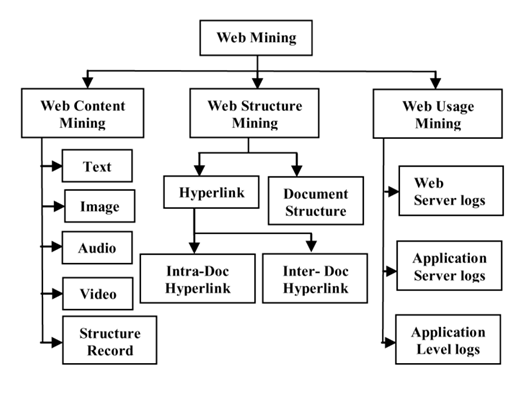
\includegraphics[width = 95mm]{webminingtax}
	\caption{Categorie di Web Mining}
	\label{webminingtax}
\end{figure}

\paragraph{Web Structure Mining}
Il Web Structure Mining � un processo di estrazione di informazioni utili partendo dalla struttura ad hyperlink di un sito Web, che viene considerato come un grafo, i cui nodi sono le pagine e gli archi sono gli hyperlink tra le pagine.
\\
Basata sulla topografia degli hyperlink, il Web Structure Mining pu� categorizzare le pagine web e generare informazioni come la similarit� e le relazioni tra i differenti siti Web \cite{Nilima}.
\\
Tecniche tradizionali di Data Mining non possono generare conoscenza utile perch� non � presente una struttura a link in una tabella relazionale (i.e. database).
\\
Tra i pi� importanti algoritmi che appartengono a questa tipologia si possono trovare Page Rank \cite{pagerankstanford} e HITS \cite{Kleinberg99}, i quali sfruttano la struttura ad hyperlink del Web per assegnare un rank alle pagine, ovvero per restituirle in ordine di importanza relativamente ad una determinata query.

\paragraph{Web Content Mining}
Il Web Content Mining viene usato per cercare informazioni utili dai contenuti delle pagine Web, che possono essere collezioni di testi, immagini, audio, video o dati strutturati incapsulati in liste e tabelle.
\\
Per estrarre il sapere da contenuti pi� complessi, come le immagini, le tecniche di Web Content Mining sono molto limitate \cite{webmining21cap}.
\\
Le tecniche di questa tipologia di Web Mining possono sembrare abbastanza simili alle metodologie tradizionali di Data Mining o di Text Mining, ma le caratteristiche delle pagine Web (e.g. presenza di tag HTML) non permette a queste di essere direttamente applicabili sulle stesse.

\paragraph{Web Usage Mining}
Il Web Usage Mining � l'applicazione delle tecniche di Data Mining per la scoperta di pattern e informazioni utili attraverso l'analisi dei log, che sono immagazzinati nei Web server o nei sistemi che tracciano le attivit� degli utenti.
\\
L'obiettivo di questo campo � la profilazione dell'utente, ovvero analizzare i suoi comportamenti sul web, sia per comprendere quali sono i suoi reali bisogni, sia per offrire dei servizi che possano soddisfare tali necessit� e personalizzare l'esperienza Web.
\\
Questo tipo di Web Mining viene usato in campi disparati, che vanno dalle aziende alle agenzie governative: ad esempio, i siti di e-commerce usano questo tipo di tecnologia per presentare all'utente prodotti per i quali potrebbe essere interessato; le agenzia governative, invece, usano il Web Mining anche per classificare minacce e attentati terroristici.
\\
Alcuni, per�, criticano questa tecnologia: il problema etico di cui pi� si parla � la violazione della privacy, con il rischio di vedere diffusi i propri dati, anche sensibili, senza alcuna consapevolezza da parte dell'utente \cite{612259}.

\section{Rappresentazioni di pagine Web}
\label{webpagerapresentation}
Un sito � formato da pagine Web. Queste sono caratterizzate da numerose rappresentazioni, che sono:

\begin{itemize}
	\item \textbf{Rappresentazione testuale}. Il testo � una componente fondamentale di una pagina Web, poich� ha come scopo il trasferimento dell'informazione. Durante la navigazione, infatti, l'utente estrapola conoscenza semplicemente leggendo il contenuto testuale delle pagine che visita.
	\item \textbf{Rappresentazione visuale}. Quando una pagina Web viene renderizzata da un browser, viene applicato uno stile di formattazione visuale, chiamato CSS, che definisce gli elementi della pagina Web come contenitori rettangolari che sono disposti o uno dopo l'altro o annidati tra loro formando un albero chiamato \texttt{Rendered Box Tree}. L'albero in questione � differente dalla struttura della pagina definita dai tag HTML, poich� una pagina pu� essere ricca di elementi invisibili, come il tag $<$head$>$ o da elementi aventi come stile $display:none$. Inoltre, la generazione del rendered box tree richiede l'esecuzione di codice JavaScript e CSS.
	\item \textbf{Rappresentazione strutturale}. Questa � composta da elementi Web inscritti in tag HTML ed organizzata ad albero. I tag HTML possono essere applicati a porzioni di testo, hyperlink e dati multimediali per fornire loro un significato ed una renderizzazione differente della pagina da parte del browser.
\end{itemize}

In particolare, trattando una pagina Web come un documento testuale, � possibile produrre una rappresentazione vettoriale mediante algoritmi di Word space model, Vector space model, Word embedding (tra cui Word2Vec) per effettuare l'apprendimento. Non solo, trattando tale testo come un paragrafo, � possibile applicare un altro algoritmo di Word embedding, ovvero Doc2Vec.
\\
Ma una pagina Web pu� anche essere trattata come un nodo del sito, il quale non � altro che un grafo, in cui i nodi sono le pagine del sito stesso e gli archi sono gli hyperlink tra i nodi. � possibile, quindi, produrre una rappresentazione vettoriale delle pagine basandosi sulla struttura ad hyperlink del sito. Un esempio � LINE.
\\
Tutti gli algoritmi e le metodologie appena citate verranno descritte nelle sezioni successive.
%L'estrazione di informazione utile, a partire da pagine Web di tipo non strutturato o semi-strutturato � un processo impegnativo.
%\\
%Un modo per affrontare questa sfida � l'applicazione di algoritmi di Machine Learning che possano individuare schemi per estrapolare informazioni utili a partire dai contenuti e dalla struttura delle pagine Web.
%\\
%Per definizione, il Machine Learning � un campo di ricerca, appartenente all'Informatica, che si occupa dello studio della scoperta di pattern. La maggior parte degli algoritmi di Machine Learning trasformano il contenuto di un testo in uno spazio vettoriale \cite{live-2934-4846-jair}, permettendo di estrapolare l'informazione nascosta da testi scritti in linguaggio umano.
%\\
%In questa tesi viene proposto l'utilizzo del modello di spazi vettoriali per rappresentare i vertici del grafo della pagina Web. Per spiegare che cos'� e perch� � importante il modello di spazio vettoriale, occorre specificare e descrivere l'argomento di quello dello spazio delle parole (Word space model), che sono strettamente collegati l'uno all'altro.

\subsection{Word space model}
Il Word Space Model, come definito in \cite{wordspacemodel}, � una rappresentazione spaziale del significato delle parole. Si basa sul fatto che la similarit� semantica viene rappresentata come prossimit�, in uno spazio ad $n$ dimensioni, dove $n$ � un intero.

\begin{figure}[h]
	\centering
	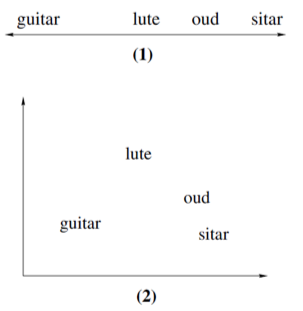
\includegraphics[width = 50mm]{wordspaceexample}
	\caption{Esempi di spazi di parole, rispettivamente mono-dimensionale (1) e bi-dimensionale (2)}
	\label{wordspaceexamples}
\end{figure}

In Figura \ref{wordspaceexamples} sono riportati due esempi di spazi di parole, in cui la prossimit� � data dalla posizione delle parole nello spazio.
In entrambi i casi, si pu� notare come il termine $sitar$ sia pi� simile di significato a $oud$, e meno simile a $guitar$.
\\
Ma come si costruisce uno spazio delle parole? Una modalit� di costruzione � la \textbf{matrice di co-occorrenze}. Tale matrice pu� essere formata sia parola per parola ($w$ x $w$), dove $w$ sono i tipi di parole nel set, sia parola per documento ($w$ x $d$), dove $d$ sono i documenti nel set. Le celle di questa matrice registrano la frequenza di occorrenza della parola i-esima in un contesto j-esimo, oppure in un documento j-esimo nel caso di matrice parola per documento.
\\\\
Per spiegare la matrice di co-occorrenze prendiamo come esempio la frase:
\begin{figure}[h]
	\centering
	Whereof one cannot speak thereof one must be silent
	\label{sentencematrix}
	\caption{Frase di esempio per la matrice di co-occorrenze \cite{wordspacemodel}}
\end{figure}

\begin{table}[h]
	\centering
	\caption{Matrice di co-occorrenze parola per parola \cite{wordspacemodel}}
	\label{tablematrix}
	\begin{tabular}{|l|l|l|l|l|l|l|l|l|}
		\hline
		& whereof & one & cannot & speak & thereof & must & be & silent  \\ \hline
		whereof & 0 & 1 & 0 & 0 & 0 & 0 & 0 & 0  \\ \hline
		one & 1 & 0 & 1 & 0 & 1 & 1 & 0 & 0 \\ \hline
		cannot & 0 & 1 & 0 & 1 & 0 & 0 & 0 & 0 \\ \hline
		speak & 0 & 0 & 1 & 0 & 1 & 0 & 0 & 0 \\ \hline
		thereof & 0 & 1 & 0 & 1 & 0 & 1 & 0 & 0 \\ \hline
		must & 0 & 1 & 0 & 0 & 1 & 0 & 1 & 0 \\ \hline
		be & 0 & 0 & 0 & 0 & 0 & 1 & 0 & 1 \\ \hline
		silent & 0 & 0 & 0 & 0 & 0 & 0 & 1 & 0 \\ \hline
	\end{tabular}
\end{table}

Le celle della matrice di co-occorrenze, visibile nella Tabella \ref{tablematrix}, registrano le occorrenze delle parola i-esima, le quali dipendono dal contesto. Con il termine \textit{contesto} si intende un insieme di parole che si trovano nelle vicinanze della parola i-esima.
\\
Queste liste di occorrenze sono dei veri e propri vettori. Un vettore, per definizione, � un elemento di uno spazio vettoriale, ed � definito da $n$ componenti o coordinate $\overrightarrow{v} = (x_1, x_2, ..., x_n)$ \cite{wordspacemodel}. Tali coordinate definiscono la posizione nello spazio n-dimensionale.
\\
Quindi, la matrice di co-occorrenze non � altro che una realizzazione del modello dello spazio vettoriale, chiamato Vector Space Model.

\paragraph{Vector Space Model}
\label{tfidf}
Il Vector Space Model � una modalit� algebrica per rappresentare documenti di testo come vettori, inseriti in uno spazio vettoriale.
\\
Generalmente, per definire i vettori viene usato come peso \textit{tf-idf}, una funzione che viene usata per misurare l'importanza di un termine rispetto ad un documento o ad una collezione di documenti. Come suggerisce il nome, � composta da due fattori: \textit{tf} e \textit{idf}.
\\
\textit{Tf}, abbreviazione di \textit{term frequency}, misura quante volte un termine appare in un documento. Dato che ogni documento ha lunghezza differente, ovvero � composto da un differente numero di parole, � possibile che un termine possa apparire molte pi� volte nei documenti pi� lunghi rispetto a quelli pi� corti. Questo problema viene risolto dividendo la frequenza dei termini per la lunghezza del documento. La formula �:
\begin{equation}
	tf_{i, j} = \frac{n_{i, j}}{|d_J|}
\end{equation}
dove $n_{i, j}$ � il numero di occorrenze del termine $t_i$ che si trova nel documento $d_j$, mentre il denominatore � la dimensione del documento $d_j$.
\\
\textit{Idf}, abbreviazione di \textit{inverse document frequency}, misura invece i termini che si presentano pi� volte in un documento, ma con meno frequenza in tutta la collezione di documenti. Questo perch� potrebbero esserci dei termini  pi� significativi che appaiono raramente in un determinato elaborato, ma frequentemente nel set di documenti. La formula �:
\begin{equation}
	idf_i = \log{\frac{|D|}{|\{d : t_i \in d\}|}}
\end{equation}
dove $|D|$ � il numero di documenti presenti nella collezione, mentre il denominatore � il numero di documenti che contengono il termine $t_i$.
\\\\
Il modello di spazio vettoriale sopra descritto, per�, presenta particolari problematiche quando si vuole costruire uno spazio delle parole: da un lato, se non si hanno sufficienti dati, non sar� possibile costruire, in maniera fedele, un modello di distribuzione delle parole; dall'altro, se tale spazio vettoriale sar� dimensionalmente grande, innalzer� la complessit� computazionale.
\\
Secondo la sperimentazione portata avanti da \cite{wordspacemodel}, � stato riscontrato un altro problema: nella matrice di co-occorrenze circa il 99\% delle celle conterr� zero come valore. Solo una parte delle parole apparir� realmente. Questo fenomeno � un esempio dell'applicazione della \textit{Zipf's law}, una legge empirica che deriva dalla frequenza di un evento $P_i$, che fa parte di un insieme, in funzione della posizione $i$ chiamata \textit{rango} nell'ordimanto decrescente rispetto alla frequenza stessa di tale evento. La formula della legge � la seguente:
\begin{equation}
	f(P_i) = \frac{c}{i}
\end{equation}
dove $i$ indica il rango, $P_i$ indica l'evento che occupa l'i-esimo rango (ovvero l'i-esimo evento pi� frequente), $f(P_i)$ � il numero di volte (frequenza) che si verifica l'evento $P_i$, c � una costante di normalizzazione, pari al valore $f(P_i)$.
\\\\
Una possibile soluzione alle situazioni problematiche sopra descritte � la riduzione della dimensione (\textit{dimensional reduction}): un processo di compressione di uno spazio multi dimensionale ad uno avente bassa dimensione, causando anche la riduzione della grandezza della matrice e del numero di zero ivi inseriti.
\\
Una tecnica di riduzione della dimensione pi� utilizzata � \textit{t-SNE}, che � particolarmente adatta per comprimere uno spazio vettoriale di grandi dimensioni in uno avente uno, due o tre dimensioni, per poi essere visualizzato in un grafico di dispersione. Questo tipo di grafico � un sistema gli assi cartesiani di uno, due o tre dimensioni. Una volta effettuata la riduzione, i valori ottenuti per ciascun elemento del set vengono usati per posizionarlo nello spazio.

\begin{figure}[h]
	\centering
	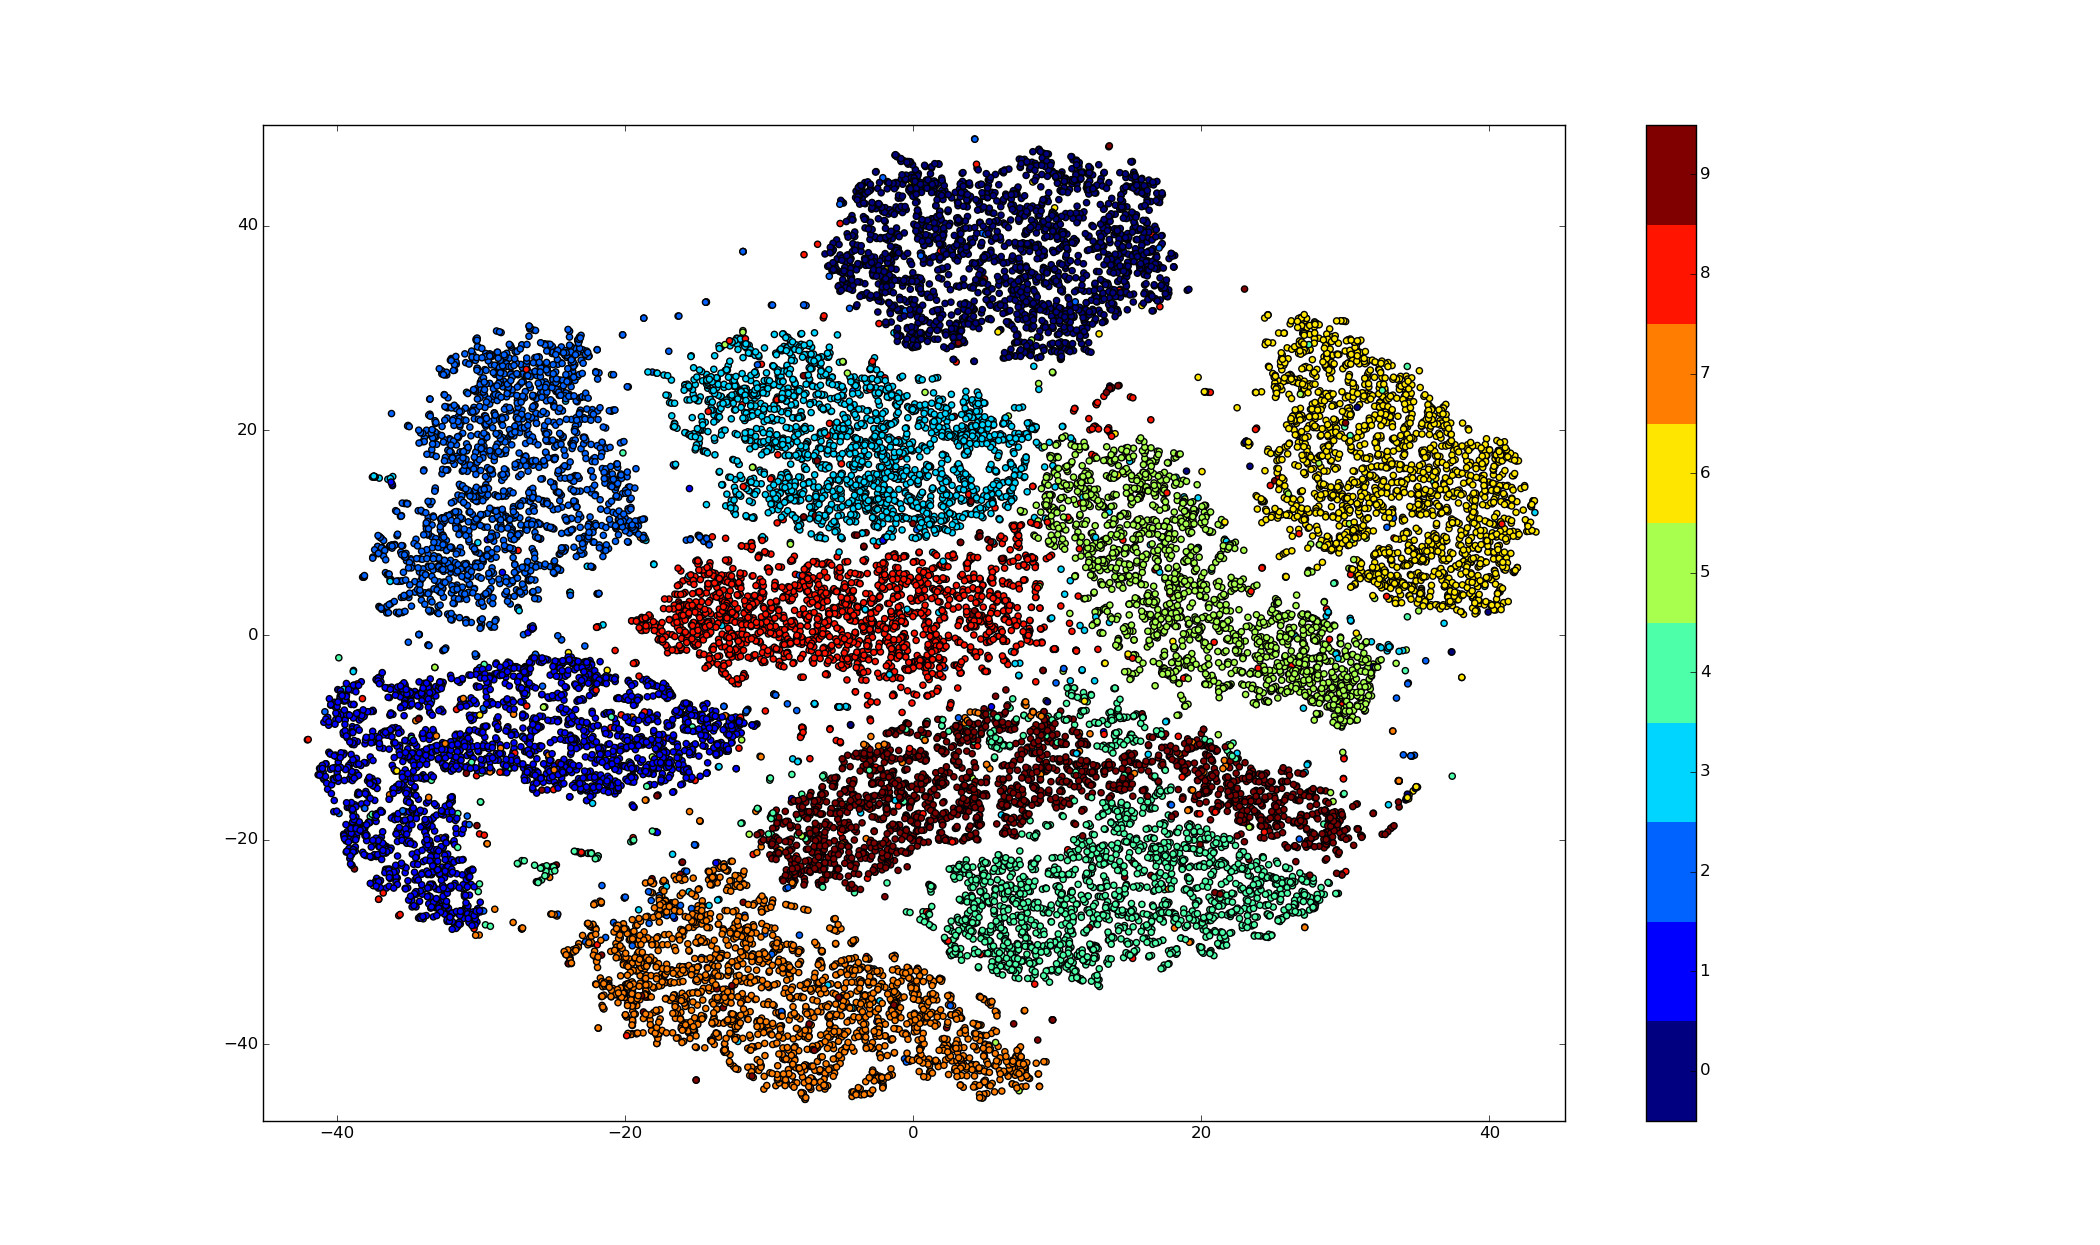
\includegraphics[width = 160mm]{tsne}
	\caption{Esempio di grafico di dispersione}
	\label{tsne}
\end{figure}

\paragraph{Word embedding}
La funzione peso \textit{tf-idf} non � la sola usata per costruire uno spazio dei vettori: nelle tecniche di Data Mining, che sfruttano gli algoritmi di Machine Learning, ci si sta orientando sempre pi� sull'uso delle reti neurali per estrarre conoscenza partendo da una collezione di dati.
\\
Questo � il Word Embedding, nome di una serie di tecniche per il language modeling e per il Feature Learning nel campo del Natural Language Processing \cite{bengio03}, in cui ad ogni parola viene associato un vettore chiamato \textit{Feature Vector}.
\\
Il Word Embedding � una funzione parametrizzata
\begin{equation}
	W : words \to \mathbb{R^n}
\end{equation}
che trasforma le parole di un dato linguaggio in un vettore multidimensionale. Per esempio:
\begin{equation}
	W("mat") = (0.0, 0.6, -0.1, ...)
\end{equation}
Partendo da un documento, � possibile trasformare i termini in vettori, formando un vero e proprio spazio vettoriale, chiamato anche Word Embeddings Space.

\begin{figure}[h]
	\centering
	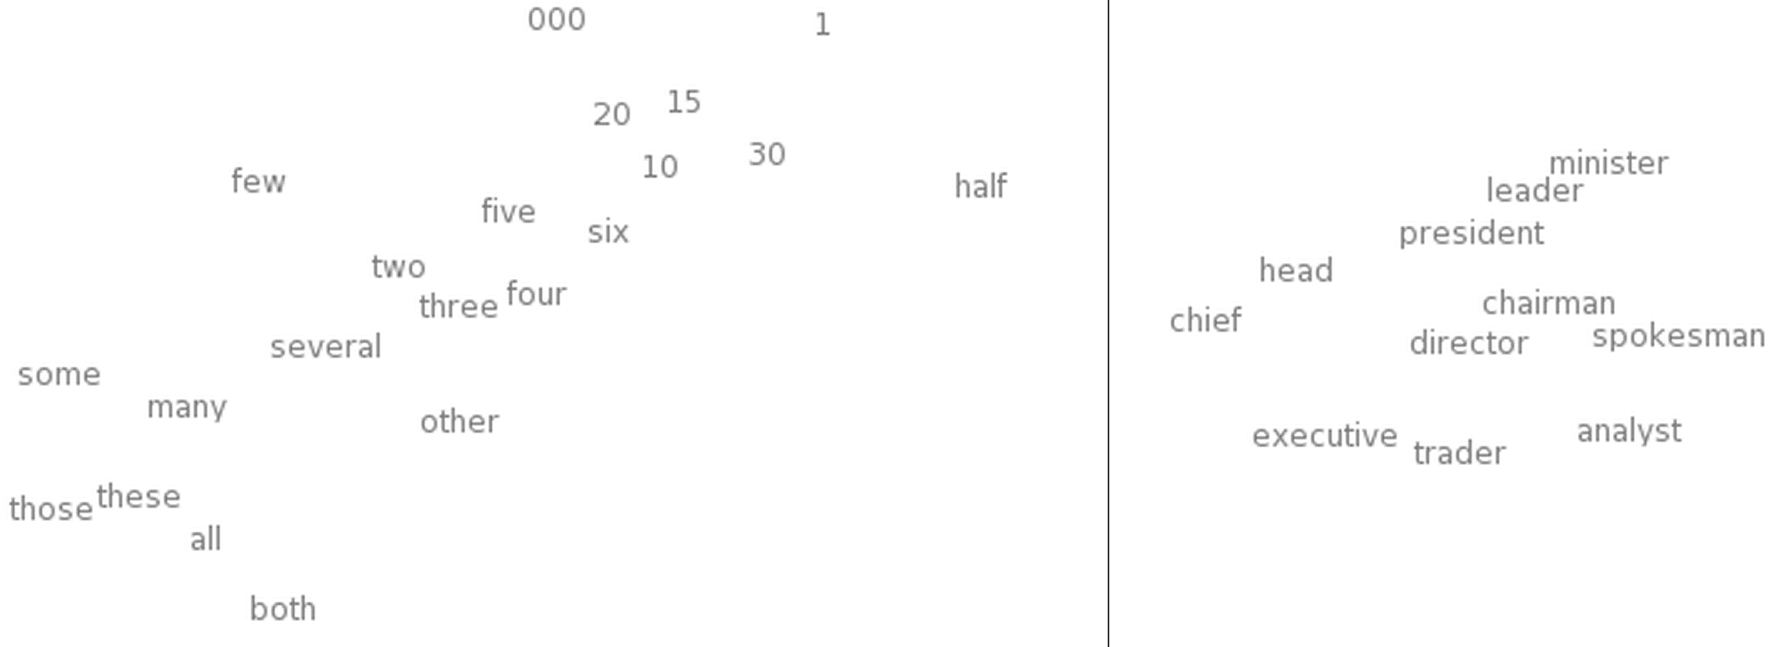
\includegraphics[width = 150mm]{tsneplot}
	\caption{Esempio di spazio degli embeddings}
	\label{tsneplot}
\end{figure}

In Figura \ref{tsneplot} � possibile notare come parole simili si trovano vicine tra loro: la parola \textit{three} � molto vicina alle parole \textit{two} e \textit{four}. Questo � dovuto al fatto che tali parole hanno vettori simili. Infatti, se si usa un sinonimo, la validit� della frase non cambia (per esempio: "poche persone cantano bene" $\to$ "un paio di persone cantano bene"), perch� le parole "poche" e "paio" sono vicine tra loro ed hanno vettori simili.
\\\\
Un'altra propriet� interessante della funzione di Word Embedding � l'analogia tra le parole, nascosta nella differenza dei loro vettori:
\begin{equation}
	W("woman") - W("man") \simeq W("queen") - W("king")
\end{equation}
Da questo si evince che c'� una correlazione tra parole che hanno genere opposto, in quanto appariranno in contesti simili, differenti solo per alcuni dettagli come pronomi o articoli. Lo stesso principio vale per parole singolari e plurali \cite{mikolov13}.
\\\\
Apprendere dei termini e trasformarli in Feature Vectors rappresenta una base per effettuare operazioni di Data Mining, come per esempio il raggruppamento dei termini appresi in gruppi attraverso il Clustering, usando qualche funzione di similarit�. Si approfondiranno tali funzioni nella Sezione \ref{distancefunctions}.

\subsection{Word2Vec}
\label{word2vec}
Word2Vec � un algoritmo di Word Embedding ed � una rete neurale a due livelli che apprende le parole da un testo in input, le quali vengono trasformate in vettori chiamati Feature Vectors. Viene considerato erroneamente come un deep-learning (apprendimento approfondito): in realt� si tratta di un apprendimento di tipo superficiale (shallow-learning).
\\\\
L'output di questa rete neurale � un vocabolario in cui ogni termine ha un vettore, che pu� essere compreso da una rete di deep-learning o semplicemente interrogato per rilevare delle relazioni tra i termini.

\begin{figure}[h]
	\centering
	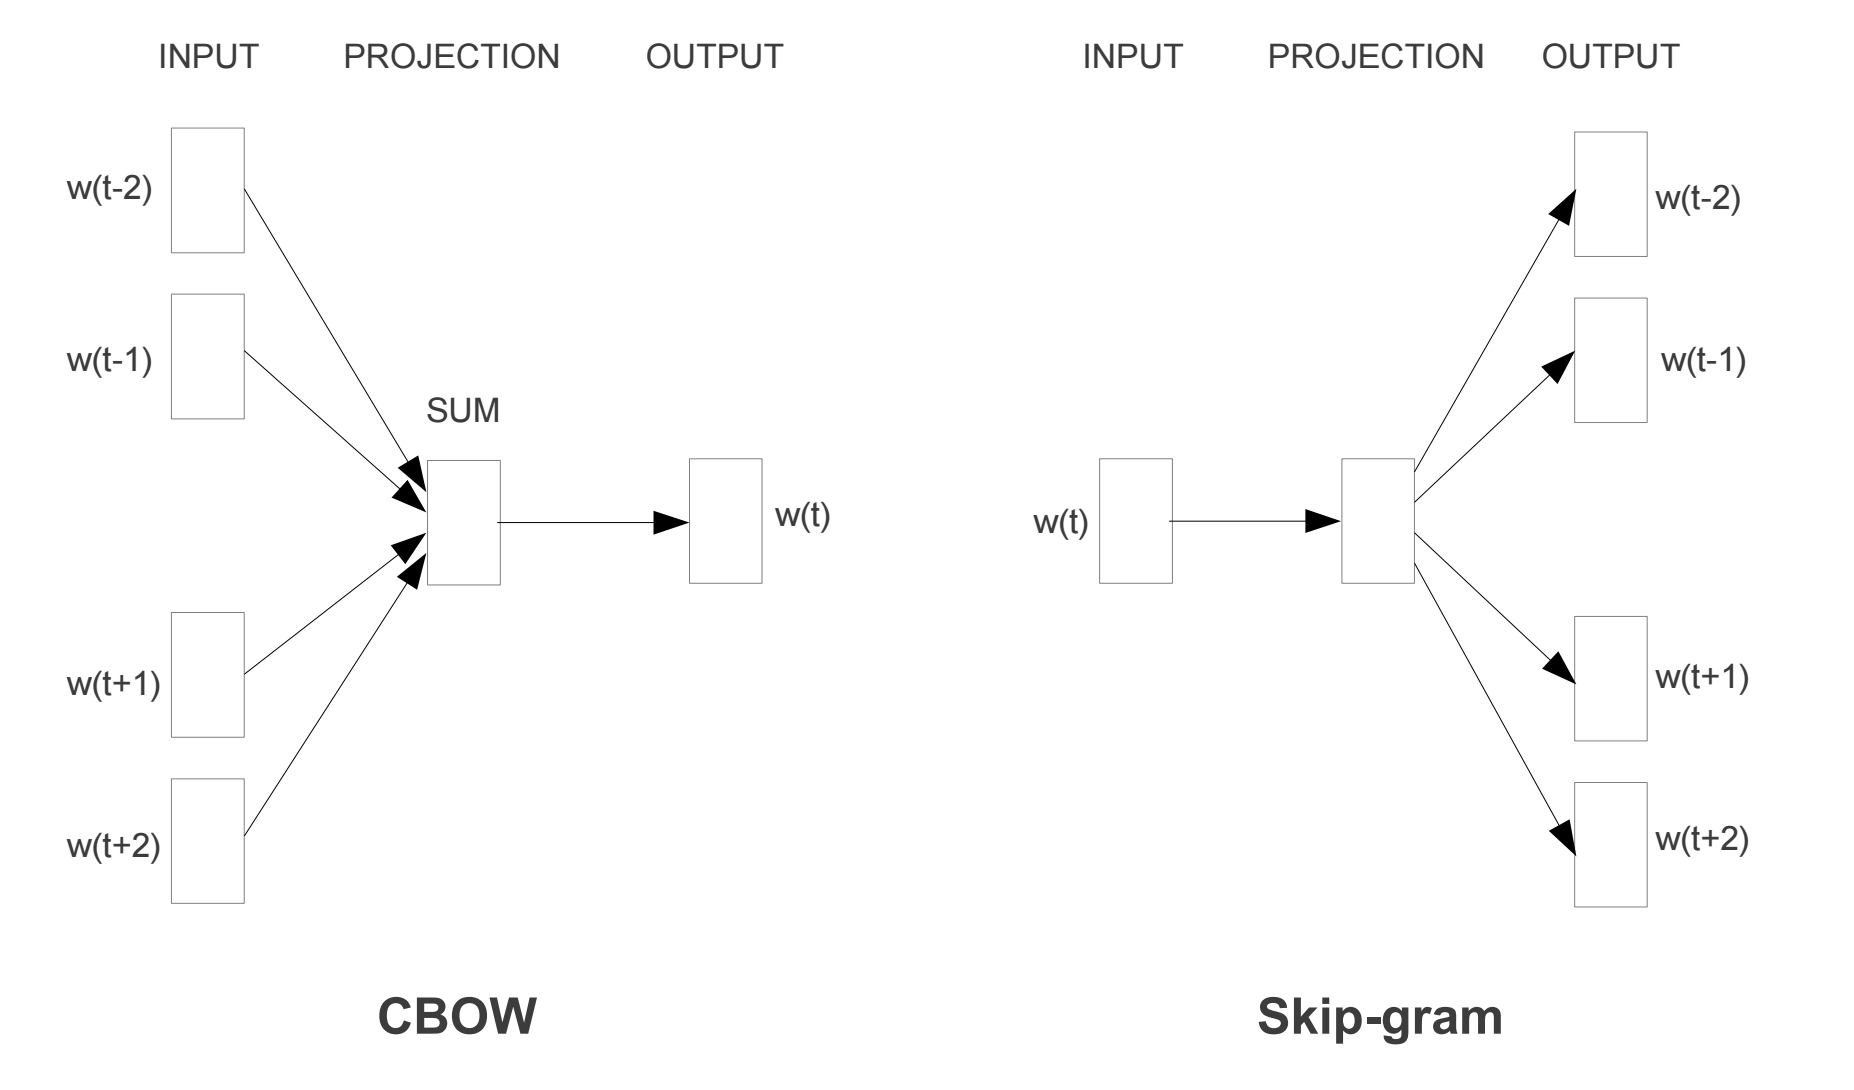
\includegraphics[width = 150mm]{word2vecmodels}
	\caption{I modelli di apprendimento di Word2Vec}
	\label{word2vecmodels}
\end{figure}

Word2Vec � composto da due modelli di apprendimento: \textbf{CBOW} (continuous bag of words) e \textbf{Skip-Gram}.
\\\\
\textbf{CBOW} consiste nel predire una determinata parola a partire dal suo contesto, che � composto dal numero di parole che vengono prese in considerazione durante l'apprendimento. Questo modello di apprendimento tratta l'intero contesto come una sola osservazione. Generalmente, CBOW restituisce risultati pi� accurati con piccole collezioni di dati \cite{mikolov}.
\\\\
\textbf{Skip-Gram}, invece, � l'inverso di CBOW: predice il contesto a partire da una parola.\\
Questo modello di apprendimento tratta ogni coppia contesto-obiettivo come una nuova osservazione, rendendo i risultati pi� accurati quando si hanno grandi collezioni di dati \cite{mikolov}.
\\
L'obiettivo dell'apprendimento di questo modello � quello di trovare le rappresentazioni vettoriali delle parole utili per predire quelle circostanti in una frase o in un documento. Formalmente, data una sequenza di parole $w_1, w_2, ..., w_T$ viene costruito un vocabolario, i cui termini hanno un vettore con $n$ dimensione generato casualmente. Skip-Gram deve massimizzare la probabilit� media logaritmica:
\begin{equation}
\label{skipgrameq}
	\frac{1}{T} \sum_{t=1}^{T} \sum_{-c \le j \le c, j \neq 0} \log p(w_{t+j}|w_t)
\end{equation}
dove $c$ � la dimensione della finestra di contesto, $w_t$ � la parola in input e $w_{t+j}$ � la parola in analisi del contesto.
\\
Per capire meglio questo tipo di modello di apprendimento, analizziamo questa frase:
\begin{figure}[h]
	\centering
	The quick brown fox jumped over the lazy dog.
\end{figure}
\\
Inizialmente, si crea il set di dati formato da coppie (contesto, parola), di cui il primo � una sequenza di parole che dipende dalla dimensione della finestra, mentre la parola � il termine che si sta esaminando. Quindi, se si ha una finestra di contesto di dimensione 1, il set di dati sar�:

\begin{figure}[h]
	\centering
	([quick], the), ([the, brown], quick), ([quick, fox], brown), [...] $\to$ (the, quick), (quick, the), (quick, brown), (brown, quick), [...]
\end{figure}

Supponiamo di trovarci al passo $t$, dove si trova il primo caso di apprendimento (the, quick). L'obiettivo � quello di predire \textit{quick} da \textit{the}, applicando la formula \ref{skipgrameq} e massimizzando la probabilit� media logaritmica per apprendere il vettore ottimale di \textit{quick}. Cos� facendo le parole simili avranno vettori simili. Ad ogni passo vengono aggiornati i vettori delle parole precedentemente apprese. Questo processo di apprendimento viene ripetuto sull'intera collezione di dati.

\subsection{Doc2Vec}
\label{doc2vec}
Doc2Vec, chiamato anche Paragraph2Vec, � un'estensione di Word2Vec che apprende correlando etichette e parole, invece che parole con altre parole.
\\
Differentemente da Word2Vec, che converte una parola in un vettore, Doc2Vec aggrega tutte le parole di un paragrafo in un vettore.
\\
Quindi, data una collezione di testi che possa essere divisa in $n$ documenti, o paragrafi, ad ogni paragrafo � assegnato un vettore. Il processo di apprendimento � caratterizzato dallo spostamento della finestra delle parole di contesto attraverso ogni parola di ogni paragrafo, per ogni paragrafo \cite{HongSeokho}.
\\
L'idea di base � quella di apprendere vettori di paragrafi in maniera simile all'apprendimento dei vettori delle parole. Vengono create due matrici: una formata dai vettori dei paragrafi appresi e l'altra da quelli delle parole. Il vettore del paragrafo � condiviso per tutte le parole che si trovano nello stesso, ma non per gli altri paragrafi. Gli embedding dei vettori e dei paragrafi sono combinati durante l'apprendimento ed aggiornati mediante la concatenazione o la media. I vettori vengono appresi utilizzando coppie, composte dalla parola da predire e dal contesto del campione, contrassegnato da un identificativo del paragrafo \cite{mirela}.
%\\
%Come Word2Vec, Paragraph2Vec ha due modelli di apprendimento:
%\begin{itemize}
%	\item \textbf{Distributed Memory}. Simile al modello CBOW di Word2Vec. Dati in input $N$ paragrafi e $M$ parole, viene casualmente inizializzata una matrice di embedding $D$ per i paragrafi ed una $W$ per le parole. Per ogni paragrafo si predice la successiva parola effettuando la media o il concatenamento dei vettori di paragrafo e dei termini nella finestra di contesto, che scorre per tutta la lunghezza del paragrafo stesso, non modificando il suo vettore. Una volta che viene completato il paragrafo, vengono aggiornate le matrici $D$ e $W$.
%	\item \textbf{Distributed Bag of Words}. Simile al modello Skip-Gram di Word2Vec. Vengono predette le parole che si trovano in un paragrafo dando solo il suo vettore. Questo modello � concettualmente pi� semplice e pi� efficiente in termini di memoria.
%\end{itemize}

\subsection{LINE}
\label{line}
LINE � un nuovo modello di apprendimento, capace di produrre rappresentazioni vettoriali (embedding) di vertici in una rete o grafo. Un grafo � una coppia ordinata $G = (V, E)$ di insiemi, con $V$ insieme dei nodi ed $E$ insieme degli archi.
\\
Questo modello di apprendimento lavora bene soprattutto con grafi orientati, pesati e non-pesati. Viene richiesto come input un file contenente gli archi che costituiscono il grafo da apprendere. L'obiettivo � quello di rappresentare ogni vertice $v \in V$ in un vettore $R^d$ applicando una funzione $f_G : V \to R^d$, dove $d << |V|$ \cite{tang2015line}. Viene prodotto, infine, uno spazio vettoriale formato da rappresentazioni vettoriali dei singoli nodi del grafo appreso.% Ogni vettore $R^d$ preserva la prossimit� di primo e secondo ordine tra i vertici.
\\
LINE preserva sia la prossimit� di primo che di secondo ordine. Nel primo caso ottimizza la seguente funzione di perdita:
\begin{equation}
\label{firstorderprox}
	- \sum_{(i,j) \in E} w_{ij} \log p_1(v_i, v_j)
\end{equation}
Trovando un insieme $\{\vec{u}_i\}_{i=1...|V|}$ che minimizza la funzione obiettivo \ref{firstorderprox}, � possibile rappresentare ogni vertice in uno spazio $d$-dimensionale. Anche nel secondo caso, si cerca di ottimizzare la seguente funzione di perdita:
\begin{equation}
\label{secondorderprox}
	- \sum_{(i,j) \in E} w_{ij} \log p_2(v_j|v_i)
\end{equation}
Trovando due insiemi $\{\vec{u}_i\}_{i=1...|V|}$ e $\{\vec{u}^{'}_i\}_{i=1...|V|}$ che minimizzano la funzione obiettivo \ref{secondorderprox}, � possibile rappresentare ogni vertice $v_i$ con un vettore $d$-dimensionale $\vec{u}_i$.

\begin{figure}[h]
	\centering
	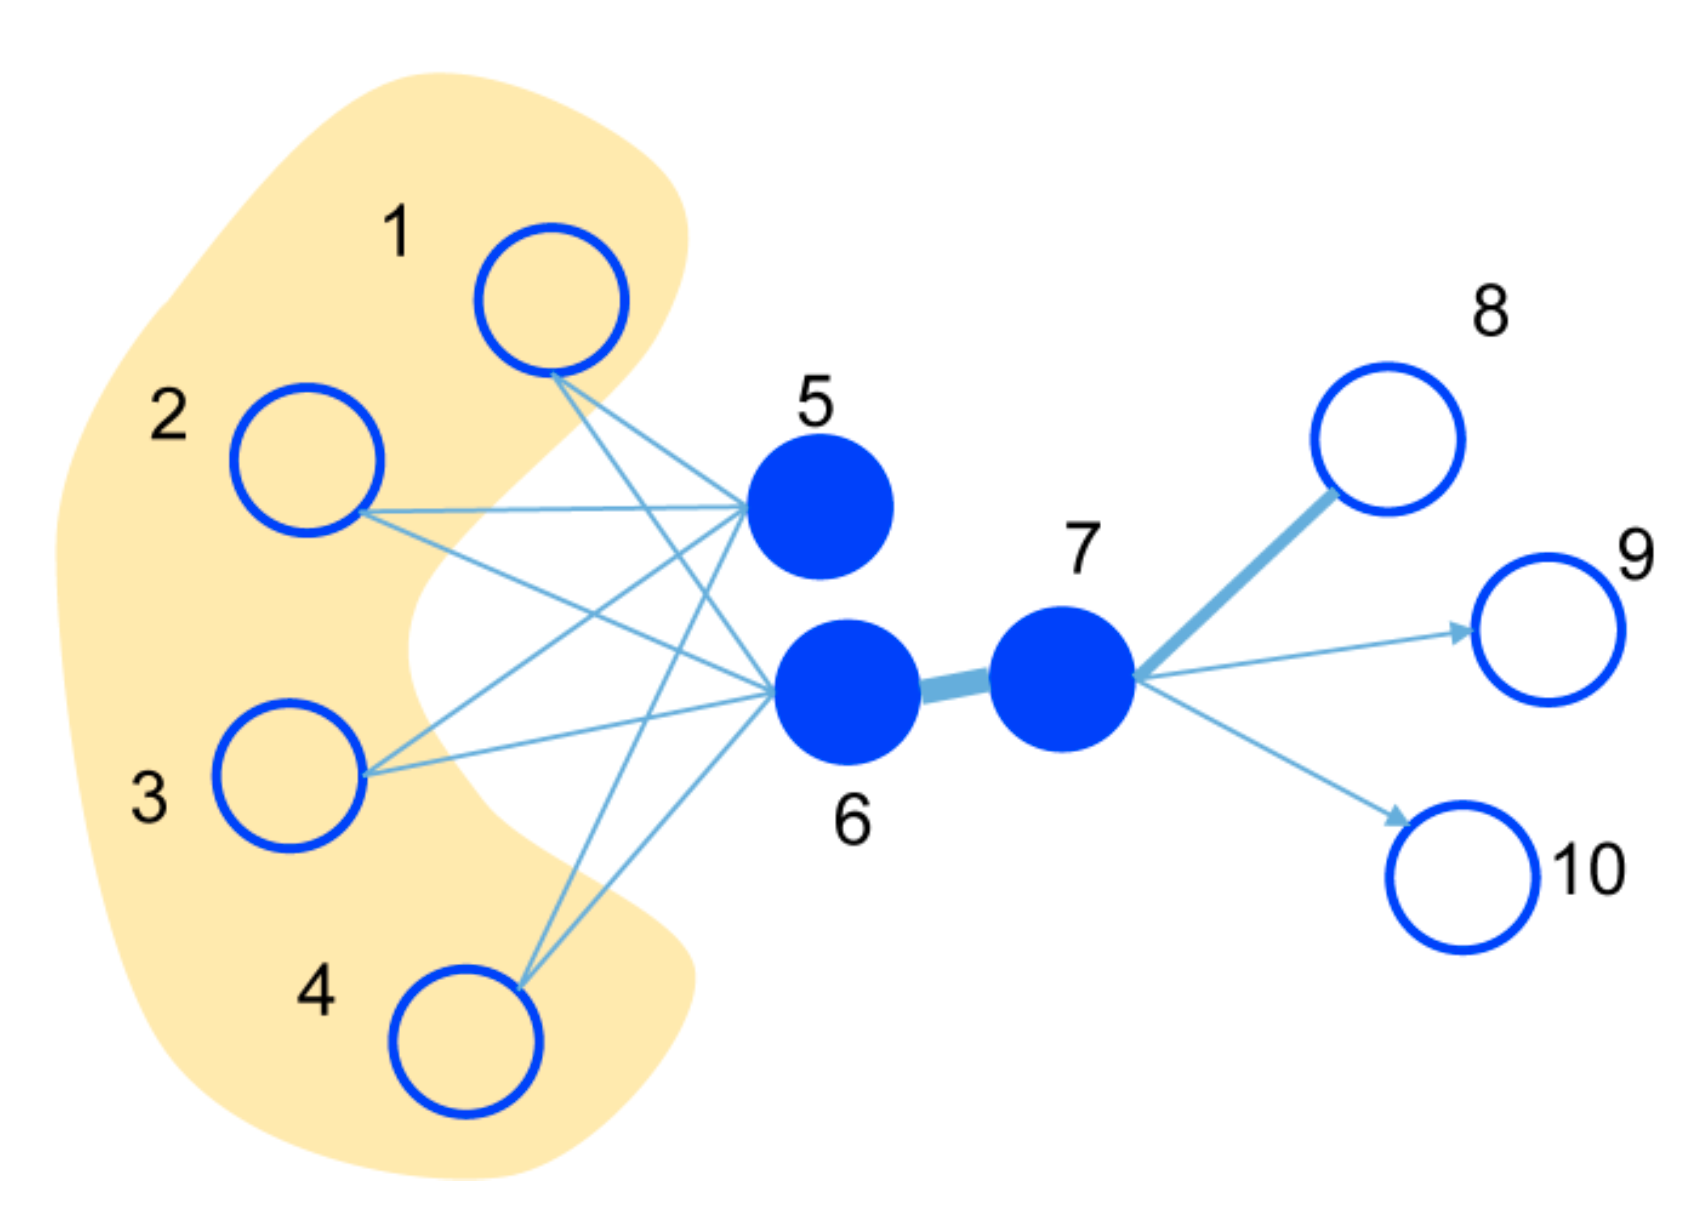
\includegraphics[width = 100mm]{infonet}
	\caption{Un esempio di grafo/network di informazioni \cite{tang2015line}}
	\label{infonet}
\end{figure}

Per spiegare la prossimit� di primo e secondo ordine, analizziamo la Figura \ref{infonet}. I vertici 6 e 7 sono collegati da un arco avente un determinato peso: tale peso indica la prossimit� di prim'ordine. Nel caso dei vertici 6 e 8, dato che non esiste un arco tra questi due, la prossimit� di primo ordine � 0.
\\
I vertici 5 e 6, invece, condividono molti vertici vicini: hanno un'alta prossimit� di secondo ordine.
\\
In altre parole, la prossimit� di primo ordine implica la somiglianza di due nodi. Per esempio, persone che sono amici gli uni con gli altri in un social network tendono a condividere simili interessi; pagine che sono collegate le une alle altre nel World Wide Web tendono a riferirsi a simili argomenti. La tipologia di secondo ordine, invece, sono persone, in un social network, che condividono simili amici che tendono ad avere simili interessi; parole che co-occorrono sempre con lo stesso insieme di termini tendono ad avere significati simili.
\\
Pu� capitare che una coppia di nodi di un grafo possa non avere un arco, avendo come prossimit� di primo ordine 0, anche essendo simili. Per questo la prossimit� di primo ordine non � sufficiente per preservare le strutture del network, ed � importante considerare una nozione alternativa di prossimit� che permetta di considerare i vertici come simili, se condividono simili nodi vicini (prossimit� di secondo ordine). LINE, quindi, permette di apprendere sia le strutture locali (i.e. i diretti vicini) sia quelli globali (i.e. i vicini dei vicini) del network.
\\
La situazione sopra descritta � riscontrabile anche in Word2Vec. Analizzare solo le parole immediatamente vicine al termine target non permette di considerare quelle simili che non si trovano vicine le une alle altre. Per questo � possibile modificare la dimensione della finestra di contesto per apprendere parole che non si trovano nell'immediato vicinato del termine target.
\\
Rispetto a LINE, che permette al pi� di analizzare i vicini dei vicini di un dato vertice (quindi relazioni avente profondit� 2), Word2Vec permette di analizzare relazioni pi� ampie, aventi profondit� maggiori di 2.
%Se due vertici hanno un'alta prossimit� dovrebbero essere rappresentati nello spazio degli embeddings vicini tra loro. Ancora, in \cite{tang2015line} si � osservato come la prossimit� di primo ordine, nel mondo reale, non � sufficiente per preservare le strutture del network globali. Per questo motivo, nella sperimentazione effettuata in \cite{tang2015line}, � stata esplorata la prossimit� di secondo ordine.
%\\
%Tali prossimit�, tuttavia, sono complementari l'una all'altra.

\section{Clustering}
\label{Clustering}
Le classi, insiemi di oggetti che condividono determinate caratteristiche, hanno un ruolo importante sia nell'analisi effettuata da persone, sia nella descrizione del mondo. Infatti, gli esseri umani hanno l'abilit� di dividere gli oggetti in gruppi e di assegnarli a questi insiemi \cite{ch8}. 
\\
Questo processo di divisione prende il nome di Clustering ed ha come scopo quello di selezionare e raggruppare, da una collezione di dati, elementi omogenei, avendo come base la somiglianza tra gli stessi.
\\
L'attivit� di raggruppamento pu� essere applicata in molti campi \cite{ch8}:
\begin{itemize}
	\item \textbf{Biologia}. Tecniche di Clustering sono state applicate per analizzare informazioni genetiche e creare una tassionomia di tutte le specie viventi.%La ricerca scientifica ha investito molto tempo per creare una tassionomia di tutte le specie viventi, basandosi sul regno, classe, ordine, famiglia, geni e specie. Non solo, tecniche di Clustering sono state applicate per analizzare una grande quantit� di informazioni genetiche: sono stati raggruppati geni che hanno funzioni simili.
	\item \textbf{Clima}. Il Clustering � stato utilizzato per trovare degli schemi nel clima della Terra.%Per capire il clima della Terra bisogna trovare degli schemi nell'atmosfera e negli oceani. Il Clustering � stato applicato per scoprirli, analizzando la pressione atmosferica delle regioni polari e nelle aree di oceano che hanno un impatto significativo sul clima della terra ferma.
	\item \textbf{Psicologia e Medicina}. Le operazioni di Clustering hanno identificato variazioni di malattie e depressioni.%Una malattia ha un incredibile numero di variazioni, e le operazioni di Clustering possono essere usate per identificare queste sottocategorie. Per esempio, � possibile applicare questo processo per scoprire tipologie differenti di depressione.
	\item \textbf{Business}. Il Clustering viene usato per dividere i consumatori in gruppi per successive attivit� di analisi e di marketing.%Il campo del Business raccoglie una quantit� enorme di informazioni di clienti potenziali ed effettivi. Il Clustering pu� essere usato per dividere i consumatori in gruppi per successive attivit� di analisi e di marketing.
	\item \textbf{Information Retrieval}. Il World Wide Web � un enorme contenitore di pagine Web, ed una semplice ricerca pu� dare come risultato milioni di pagine. Le tecniche di Clustering vengono usare per dividerle in gruppi, ognuno dei quali cattura un aspetto particolare dell'interrogazione. Quindi, se si cerca, con un motore di ricerca, la parola \textit{film}, verranno restituite pagine Web raggruppate in categorie come recensioni, trailer, celebrit�, teatri e cinema. Ogni categoria (cluster) pu� essere diviso in sottogruppi (sottocluster) e si produrr� una struttura gerarchica che servir� all'utente per effettuare altre ricerche.
\end{itemize}

%\subsection{Approcci di Clustering}
Quindi, l'operazione di Clustering � essenzialmente la creazione di un insieme di Cluster (i.e. un insieme di insiemi), che generalmente contengono tutti gli elementi iniziali.
\\
In questa tesi sono stati utilizzati algoritmi di Clustering che si basano sulla rappresentazione vettoriale degli elementi (i.e. pagine di un sito Web) per poter raggrupparli in insiemi.
\\
Esistono vari approcci di Clustering per raggruppare elementi in insiemi. Alcuni di questi sono:
\begin{itemize}
    \item Hard Clustering o Soft Clustering
    \item Partizionali o gerarchici
\end{itemize}

\paragraph{Hard Clustering e Soft Clustering}
Questi algoritmi attuano un approccio secondo cui un elemento pu� essere assegnato ad un solo Cluster o a pi� Cluster. Con Hard Clustering intendiamo che l'algoritmo assegna un elemento ad uno ed un solo Cluster; con Soft Clustering, invece, l'elemento pu� essere assegnato a pi� Cluster con gradi di appartenenza diversi.

\paragraph{Clustering partizionale}
Gli algoritmi di Clustering partizionali creano una divisione delle osservazioni minimizzando una certa funzione di costo:
\begin{equation}
   {\textstyle \sum_{j=1}^{k}} E(C_j)
\end{equation}
dove $k$ � il numero desiderato di Cluster, $C_j$ � il j-esimo Cluster ed $E : C \to \mathbb{R^+}$ � la funzione di costo associata al singolo Cluster. L'algoritmo pi� famoso che fa parte di questa categoria � K-Means.

\paragraph{Clustering gerarchico}
Gli algoritmi che fanno parte di questa categoria non suddividono lo spazio, bens� costruiscono una gerarchia di Cluster. In questa strategia rientrano due sottotipi:
\begin{itemize}
\item \textbf{Aggregativo}: tale approccio considera $n$ Cluster per $n$ elementi, cio� ogni elemento viene considerato un Cluster a s�. Successivamente, l'algoritmo unisce tutti i Cluster pi� vicini. Viene anche chiamato bottom-up.
\item \textbf{Divisivo}: tale approccio opera in maniera opposta rispetto al precedente, poich� tutti gli elementi vengono considerati come un unico Cluster e l'algoritmo deve dividere il Cluster in insiemi aventi dimensioni inferiori. Questa metodologia viene anche chiamata top-down.
\end{itemize}
Durante l'aggregazione degli elementi � necessario usare una funzione che permette di calcolare la similarit� (o meglio la distanza) tra due Cluster: questo permette all'algoritmo di unire i Cluster simili. 

\subsection{Funzioni (o misure) di distanza}
\label{distancefunctions}
A seconda dell'approccio utilizzato, vi sono delle funzioni (o misure) che permettono di calcolare la distanza tra due Cluster. Viene molto usato dagli algoritmi di Clustering gerarchico per calcolare la similarit� tra i Cluster e per unire, eventualmente, i Cluster simili.\\
Le funzioni di distanza usate da questo tipo di Clustering sono:
\begin{itemize}
	\item \textbf{Single-link proximity}. Questa funzione calcola la distanza tra due Cluster come la distanza minima tra elementi appartenenti a Cluster differenti.
	\begin{equation}
    	D(C_i, C_j) = min_{x \in C_i, y \in C_j} d(x, y)
	\end{equation}
	\begin{figure}[h!]
		\centering
		\includegraphics[width = 50mm]{Clustering_single}
		\caption{Prossimit� di tipo Single-link}
		\label{single}
	\end{figure}
	
	\item \textbf{Average-link proximity}. Questa funzione calcola la distanza tra due Cluster come la media delle distanze tra i singoli elementi.
	\begin{equation}
    	D(C_i, C_j) = \frac{1}{(|C_i||C_j|)} \sum_{x \in C_i, y \in C_j} d(x, y)
	\end{equation}
	\begin{figure}[h!]
		\centering
		\includegraphics[width = 50mm]{Clustering_average}
		\caption{Prossimit� di tipo Average-link}
		\label{average}
	\end{figure}
	
	\item \textbf{Complete-link proximity}. Questa funzione calcola la distanza tra i due Cluster, considerando la distanza massima tra gli elementi appartenenti ai due Cluster.
	\begin{equation}
		D(C_i, C_j) = max_{x \in C_i, y \in C_j} d(x, y)
	\end{equation}
	\begin{figure}[h!]
		\centering
		\includegraphics[width = 50mm]{Clustering_complete}
		\caption{Prossimit� di tipo Complete-link}
		\label{complete}
	\end{figure}
	
	\item \textbf{Distanza tra centroidi}. Questa, invece, � la distanza tra i due Cluster prendendo in considerazione i centroidi degli stessi. Un centroide � un punto rappresentativo, prodotto dalla posizione media aritmetica della distanza tra tutti i punti.
	\begin{equation}
    	D(C_i, C_j) = d\left ( \hat{c_i}, \hat{c_j} \right )
	\end{equation}
	\begin{figure}[h!]
		\centering
		\includegraphics[width = 50mm]{Clustering_centroid}
		\caption{Distanza tra centroidi}
		\label{centroid}
	\end{figure}
\end{itemize}

Nei casi precedenti, $d(x, y)$ indica una qualsiasi funzione distanza, su uno spazio metrico. Le pi� importanti sono:
\begin{itemize}
	\item \textbf{Distanza euclidea}: chiamata anche norma 2, � la distanza calcolata tra due punti, che pu� essere misurata su uno spazio multidimensionale. Siano $P = (p_1, p_2, ..., p_n)$ e $Q = (q_1, q_2, ..., q_n)$ due punti, la distanza sar�:
    \begin{equation}
        \sqrt{(p_1 - q_1)^2 + (p_2 - q_2)^2 + ... + (p_n - q_n)^2} = \sqrt{\sum_{k=1}^{k} (p_k - q_k)^2}
    \end{equation}

	%\item \textbf{Distanza di Manhattan}: chiamata anche geometria del taxi o norma 1, � la distanza tra due punti calcolata come la somma del valore assoluto delle differenze delle loro coordinate. Siano $P_1 = (x_1, y_1)$, $P_2 = (x_2, y_2)$ due punti, la distanza sar�:
    %\begin{equation}
    %    L_1(P_1, P_2) = |x_1 - x_2| + |y_1 - y_2|
    %\end{equation}

	\item \textbf{Coseno di similarit�}: tecnica euristica usata per misurare la distanza tra due vettori, che viene effettuata calcolando il coseno dell'angolo ivi compreso, che hanno l'origine coincidente con quello del sistema di assi e passano per i rispettivi elementi. Il valore risultante pi� sar� vicino ad 1, pi� i due elementi saranno simili tra loro. Siano A e B due vettori di attributi numerici, allora il coseno di similarit� sar� calcolato mediante la formula:
    \begin{equation}
        \cos(\theta) = \frac{AB}{||A|| ||B||}
    \end{equation}

	%\item \textbf{Distanza di Hamming}: misura il numero di sostituzioni necessarie per convertire una stringa nell'altra, oppure pu� essere vista come un reporting del numero degli errori che hanno trasformato una stringa nell'altra. La distanza di Hamming tra 10{\color{red}1}1{\color{red}1}01 e 10{\color{red}0}1{\color{red}0}01 � 2; oppure tra 2{\color{red}14}3{\color{red}8}96 e 2{\color{red}23}3{\color{red}7}96 � 3.
\end{itemize}

\subsection{Algoritmi usati}
\label{Clusteringexperimentation}
In questa sezione vengono descritti gli algoritmi di Clustering usati in questa tesi, che sono stati applicati per raggruppare pagine di un sito Web. Questi algoritmi si basano sulla rappresentazione vettoriale delle pagine (Sezione \ref{webpagerapresentation}) per assegnare gli elementi ad un Cluster.

\paragraph{K-Means}
K-Means � un algoritmo di Clustering di tipo partizionale, in cui ogni Cluster viene identificato mediante un centroide.
\\
Si basa sull'algoritmo di Lloyd e consiste in 3 step. Il primo step consiste nella scelta dei centroidi iniziali che saranno $K$ elementi, casuali o usando informazioni euristiche, scelti dal dataset. Successivamente, l'algoritmo assegna per ogni elemento il centroide pi� vicino e ne crea di nuovi dalla media di tutti i campioni, assegnati ai centroidi precedenti. Si ripete questa fase finch� l'algoritmo non converge.\\
Il pregio principale di questo algoritmo � la rapidit� di convergenza: si � analizzato, infatti, che il numero di iterazioni che l'algoritmo esegue � minore del numero di elementi del dataset.\\
K-means, per�, pu� essere molto lento nel caso peggiore e non garantisce il raggiungimento dell'ottimo globale: la bont� della soluzione dipende dal set di Cluster iniziale. Inoltre, un altro svantaggio � che l'algoritmo richiede, in input, il numero dei Cluster.

\begin{figure}[h]
	\centering
	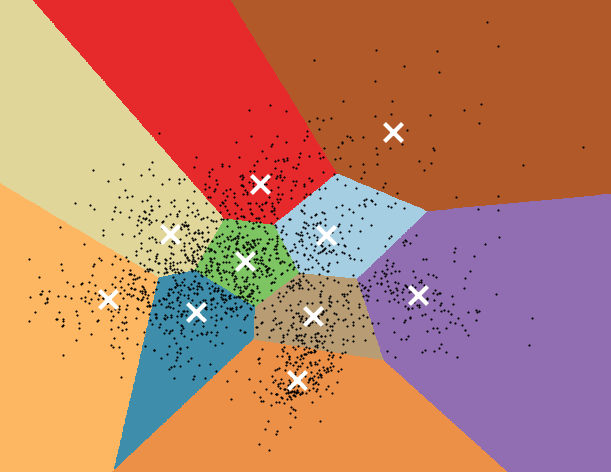
\includegraphics[width = 100mm]{kmeans}
	\caption{Esempio di Clustering utilizzando K-Means}
	\label{kmeans}
\end{figure}

\paragraph{HDBScan}
HDBScan � un algoritmo di Clustering che estende DBScan, rendendolo di tipo gerarchico.
\\
DBScan necessita di due parametri: $\epsilon$ e del numero minimo di elementi richiesti per formare un Cluster (minPts). Si comincia con un punto casuale che non � stato ancora visitato. Viene calcolato il suo $\epsilon$-vicinato, e se contiene un numero sufficiente di punti viene creato un nuovo raggruppamento. Se ci� non avviene, il punto viene etichettato come rumore, ovvero non viene associato ad alcun Cluster. � possibile che tale elemento rumore venga ritrovato in un $\epsilon$-vicinato sufficientemente grande e, quindi, inserito in un altro Cluster. Se un punto � associato ad un raggruppamento, allora anche tutti quelli nel suo $\epsilon$-vicinato sono parte del Cluster. Di conseguenza, tutti i punti trovati all'interno del suo $\epsilon$-vicinato sono aggiunti al Cluster, cos� come i loro $\epsilon$-vicini. Questo processo continua fino a quando il Cluster viene completato. Allora, un nuovo punto non visitato viene estratto e processato.

\begin{figure}[h]
	\centering
	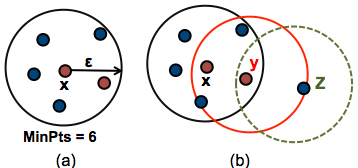
\includegraphics[width = 65mm]{dbscan}
	\caption{Principio su cui si basa DBScan}
	\label{dbscan}
\end{figure}

In HDBScan, invece, si parte in maniera simile a DBScan: lo spazio viene trasformato a seconda della densit� e viene effettuato su di esso una prossimit� a single-link. Invece di richiedere come input il parametro $\epsilon$, che viene usato da DBScan per considerare gli elementi del vicinato appartenenti al Cluster, viene creato un albero, il quale viene usato per selezionare i Cluster pi� stabili e persistenti. Viene solo richiesta la dimensione minima dei Cluster per determinare quali gruppi non devono essere considerati come Cluster, oppure per dividerli e formare nuovi Cluster.
\\
Questo algoritmo � molto efficace ed � pi� veloce sia di DBScan che di K-Means.

\section{Obiettivi della tesi}
Questa tesi ha due obiettivi:
\begin{enumerate}
	\item Capire se, combinando diverse rappresentazioni di cui una pagina Web si compone in uno spazio vettoriale al fine di applicare i tradizionali algoritmi di Clustering, vi � un miglioramento della qualit� dei Cluster prodotti.
	
	\item Verificare che, se analizzando la topologia del grafo del sito Web e dando pi� importanza a pagine vicino alla homepage, si ottengono risultati migliori rispetto all'approccio che analizza tutte le pagine come ugualmente importanti. La modifica applicata verr� discussa nella Sezione \ref{modifiedSkipgram}.
\end{enumerate}

\bibliographystyle{plain}
\bibliography{./Bibliografia}                % database di biblatex

\end{document}